\documentclass{ximera}

\usepackage{todonotes}

\newcommand{\RR}{\mathbb R}
\renewcommand{\d}{\,d}
\newcommand{\dd}[2][]{\frac{d #1}{d #2}}
\renewcommand{\l}{\ell}
\newcommand{\ddx}{\frac{d}{dx}}
\newcommand{\dfn}{\textbf}
\newcommand{\eval}[1]{\bigg[ #1 \bigg]}
\renewcommand{\epsilon}{\varepsilon}
\newcommand{\p}[1]{\left(#1\right)}
\newcommand{\br}[1]{\left[#1\right]}
\newcommand{\set}[1]{\left\{#1\right\}}


\let\prelim\lim
\renewcommand{\lim}{\displaystyle\prelim}

\colorlet{textColor}{black} 
\colorlet{background}{white}
\colorlet{penColor}{blue!50!black} % Color of a curve in a plot
\colorlet{penColor2}{red!50!black}% Color of a curve in a plot
\colorlet{penColor3}{red!50!blue} % Color of a curve in a plot
\colorlet{penColor4}{green!50!black} % Color of a curve in a plot
\colorlet{penColor5}{orange!80!black} % Color of a curve in a plot
\colorlet{fill1}{blue!50!black!20} % Color of fill in a plot
\colorlet{fill2}{blue!10} % Color of fill in a plot
\colorlet{fillp}{fill1} % Color of positive area
\colorlet{filln}{red!50!black!20} % Color of negative area
\colorlet{gridColor}{gray!50} % Color of grid in a plot


\newcommand{\fullwidth}{}
\newcommand{\normalwidth}{}



%% makes a snazzy t-chart for evaluating functions
\newenvironment{tchart}{\rowcolors{2}{}{background!90!textColor}\array}{\endarray}


\author{Gregory Hartman \and Matthew Carr}
\license{Creative Commons 3.0 By-NC}
\acknowledgement{https://github.com/APEXCalculus}

\begin{document}
\begin{exercise}

\outcome{Calculate limits using the limit laws.}
\outcome{Calculate limits of piecewise functions.}

\tag{limit} 
\tag{piecewise} 
\tag{continuous}

 Find 
  \[
  \lim_{x\to 3} f(x)
  \begin{prompt}
  = \answer{7}.
  \end{prompt}
  \]
  where
  \[
  f(x) = \left\{\begin{array}{cl} x^2-x+1 & x\leq 3, \\ 2x+1 & x>3. \end{array}\right.
  \]
    \begin{hint}
     Both pieces of $f(x)$, $x^2-x+1$, for $x\leq3$, and $2x+1$, for $x>3$, are continuous for all $x$. However, for the limit $\lim_{x\to3}f(x)$ to exist, both the left-hand and the right-hand limits of $f(x)$ at $3$ must exist and be equal.
    \end{hint}
     \begin{hint}
    	Take a look at the graph of the function
    \begin{center}
     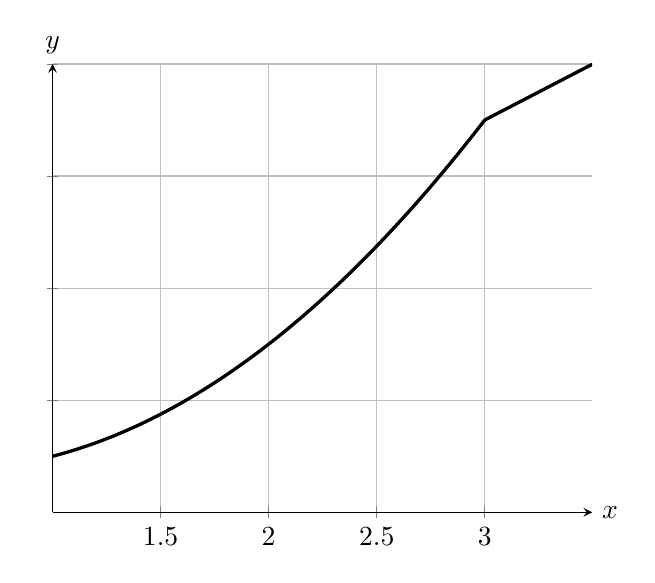
\begin{tikzpicture}
	\begin{axis}
	[ymin=0,ymax=8, axis lines=center,xlabel=$x$,ylabel=$y$,every axis y 
	label/.style={at=(current axis.above origin),anchor=south},every axis x label/.style={at=(current axis.right of origin),anchor=west},
	domain=-1:4,
	yticklabels={},
	ymajorgrids=true,
	grid = major
	]
	\addplot[domain=1:5,very thick,smooth,samples=600]
	{(!(\x>3))*(\x^2-\x+1)+(\x>3)*(2*\x+1)};
	\end{axis}
       \end{tikzpicture}      
      \end{center} 
    \end{hint}
    \begin{hint}
     Evaluating $\lim_{x\to3^{+}}f(x)$ we see that it is equal to $7$. This follows because, for $x>3$, we are on the piece of $f(x)$ given by $2x+1$ and the limit $\lim_{x\to3}\p{2x+1}=2\cdot\lim_{x\to 3}\p{x}+\lim_{x\to3}\p{1}=7$, certainly. On the other hand, evaluating $\lim_{x\to3^{-}}f(x)$ we see it is equal to $7$. This follows because, for $x\leq3$, we are on the piece of $f(x)$ given by $x^2-x+1$ and the limit $\lim_{x\to3}\p{x^2-x+1}=\p{\lim_{x\to3}\p{x}}^2-\lim_{x\to 3}\p{x}+\lim_{x\to3}\p{1}=7$, certainly. These are equal, so the limit exists is equal to $7$.
    \end{hint}
\end{exercise}

\end{document}